\documentclass[]{report}

% All Dependencies

\usepackage{graphicx}
\usepackage{float}
\usepackage{amsmath}
\usepackage{amsfonts}
\usepackage{wasysym}
% Title Page
\title{MATH 4820 - Homework 2}
\author{Jack Reilly Goldrick}


\begin{document}
	\maketitle
	
	
\section{Problem 1 using Area of Squares}
	
	\begin{itemize}
		\item Assume $\sqrt{3} = \frac{m}{n} : m > n \ \forall m,m \in \mathbb{Z}$, and m,n are co-prime
		
		\item squaring both sides and multiplying them by $n^2$ we have:
		
						$$ 3n^2 = m^2 $$
						
						
		\item Since the area of a square is the side-length squared, this equation can be interpreted as the area of the sum three squares with side-length n is equal to the area of a square with side-length m. 
		
			\begin{itemize}
				\item This implies the larger area is divisible by three, thus, we have
				
				$$ m = 3k, \forall k \in \mathbb{Z} $$
				
			\end{itemize}
			
			
			
			
			\item Substituting 2k for m we have:
			
			$$ 3n^2 = 9k^2 $$
			
			$$ n^2 = 3k^2 $$
			
			
			\begin{itemize}
				
				\item This implies that n is also divisible by three as well.
				
		\end{itemize}
		
		
		\item The original assumption was that these numbers m and n were co-prime to satisfy $\sqrt{3}$ as a rational number.  However, we have just shown that m and n are not co-prime for the numbers m and n to remain integers.  Thus we have raised a contradiction arising from the square root of three's rationality; therefor, the square root of three is irrational.   
	\end{itemize}
	
	\begin{flushright}
		\smiley{}
	\end{flushright}
	
\section{Problem 2}

	\begin{itemize}
		\item Let $ a = 270 \land b = 168 $
		
		\item Following the Euclidean Algorithm we have:
		
		$$ 270 = q_{1}(168) + r_1  \implies q_1 = 1 \land r_1 = 102 $$ 
		
		$$ 168 = q_{2}(102) + r_2 \implies q_2 = 1 \land r_2 = 66 $$
		
		$$ 102 = q_3(66) + r_3 \implies q_3 = 1 \land r_3 = 36 $$
		
		$$ 66 = q_4(36) + r_4 \implies q_4 = 1 \land r_4 = 30 $$
		
		$$ 36 = q_5(30) + r_5 \implies q_5 = 1 \land r_5 = 6 $$
		
		$$  30 = q_6(6) + r_6 \implies q_6 = 5 \land r_6  = 0 $$
		
		
		\item This implies the gcd(270, 168) = 6
		
		\item Now to find the integer solution we have:
		\begin{align*}
		 6 &= 36 - (1 * 30)  \\
		 &= 2(36) - 66  \\		
		 &= 5(102) - 1(168)  \\
		  &= 5(270) - 6(168) 
	\end{align*}
		\item This implies $ x = 5 \land y = -6 $ 
		
	\end{itemize}
	
	
	\begin{flushright}
		\smiley{}
	\end{flushright}
	
	
	
\section{Problem 3}


	\begin{figure}[H]
		\centering
		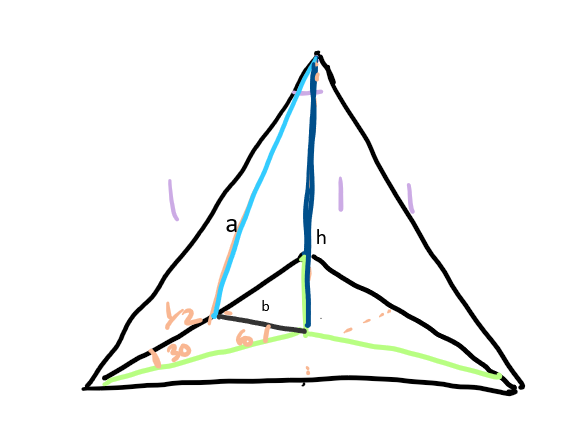
\includegraphics[width=0.7\linewidth]{pics/p3}
	\end{figure}
	
	\begin{itemize}
		\item Using my Diagram and the properties of 30-60-90 Right Triangles, we have:
		
		$$ h = \sqrt{ \frac{27}{36} - \frac{3}{36} } = \frac{\sqrt{6}}{3}  $$
	\end{itemize}

	\begin{flushright}
		\smiley{}
	\end{flushright}
	

	
	
\end{document}          
